\section{必修一知识点回顾【注意应用的数学思想:分类讨论、数形结合、变量替换】}
\subsection{集合是什么?怎么表示?有什么性质?记住一些特殊的集合及其表示方法、性质。}
    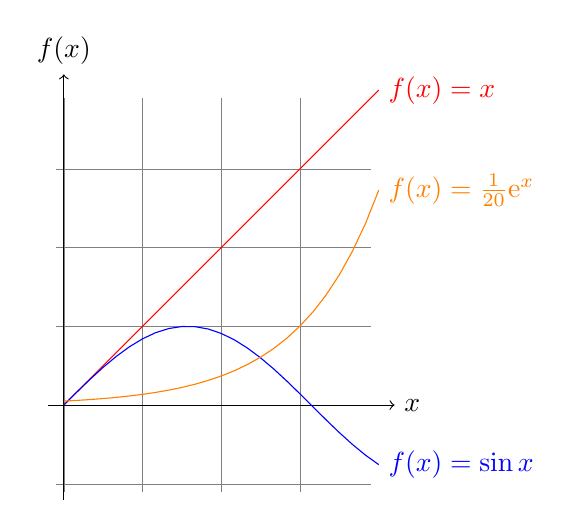
\begin{tikzpicture}[domain=0:4]
  \draw[very thin,color=gray] (-0.1,-1.1) grid (3.9,3.9);
  \draw[->] (-0.2,0) -- (4.2,0) node[right] {$x$};
  \draw[->] (0,-1.2) -- (0,4.2) node[above] {$f(x)$};
  \draw[color=red]    plot (\x,\x)             node[right] {$f(x) =x$};
  % \x r 表示弧度
  \draw[color=blue]   plot (\x,{sin(\x r)})    node[right] {$f(x) = \sin x$};
  \draw[color=orange] plot (\x,{0.05*exp(\x)}) node[right] {$f(x) = \frac{1}{20} \mathrm e^x$};
\end{tikzpicture}
\subsection{集合间有什么关系?注意与一些特殊集合间的关系。}

\begin{enumerate}
\item 集合间的运算: 交集、并集、补集的含义与表示。运算结果有何特殊性质? 
\end{enumerate}

\begin{enumerate}
\item  计算二重积分~$\ds{\iint\limits_{D}\me^{x^2+y^2}\dif \sigma}$, 其中~$D=\{(x,y)\Big| x^2+ y^2 \leqslant 25\}$.\\
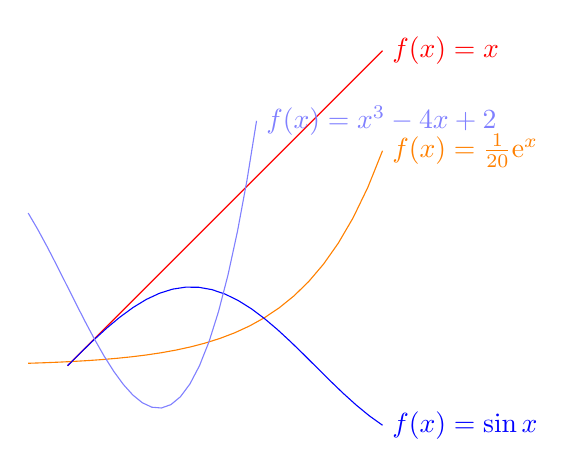
\begin{tikzpicture}[domain=0:4]
\tkzInit[xmax=4.2,ymax=3.2,xmin=-1.2,ymin=-1.2,xstep=1]
%\tkzGrid
\tkzAxeXY
\draw[color=red] plot (\x,\x) node[right] {$f(x)=x$};
\draw[color=orange,domain=-0.5:4] plot (\x,{0.05*exp(\x)}) node[right] {$f(x)=\frac{1}{20}\mathrm e^x$};
\draw[color=blue,domain=0:4] plot (\x,{sin(\x r)}) node[right] {$f(x)=\sin x$};
\draw[color=blue!50,x=1cm,y=0.5cm,domain=-0.5:2.4] plot (\x, {(\x)^3-4*(\x)+2}) node[right] {$f(x)=x^3-4x+2$};
\end{tikzpicture}
\end{enumerate}


集合的应用。集合与其他数学概念的联系。

函数是什么?怎么表示?有什么性质?记住一些特殊的函数及其表示方法、性质。\\
指数幂如何表示与计算?运算规则如何?与已学过运算间的联系?\\
对数如何表示与计算?运算规则如何?与已学过运算间的联系?

函数间有什么关系?

函数间的运算:加减乘除、复合的含义与表示。运算结果有何特殊性质?

函数的应用。函数与其他数学概念的联系。

二、运算与技巧
几种常用的表达式化简与处理办法\\
函数是什么?怎么表示?有什么性质?记住一些特殊的函数及其表示方法、性质。\\
指数幂如何表示与计算?运算规则如何?与已学过运算间的联系?\\
对数如何表示与计算?运算规则如何?与已学过运算间的联系?
几种方程与不等式的求解办法

几种常见问题含义












